\documentclass[tikz,border=14pt]{standalone}
\usepackage{tikz}
\usetikzlibrary{calc}

\begin{document}
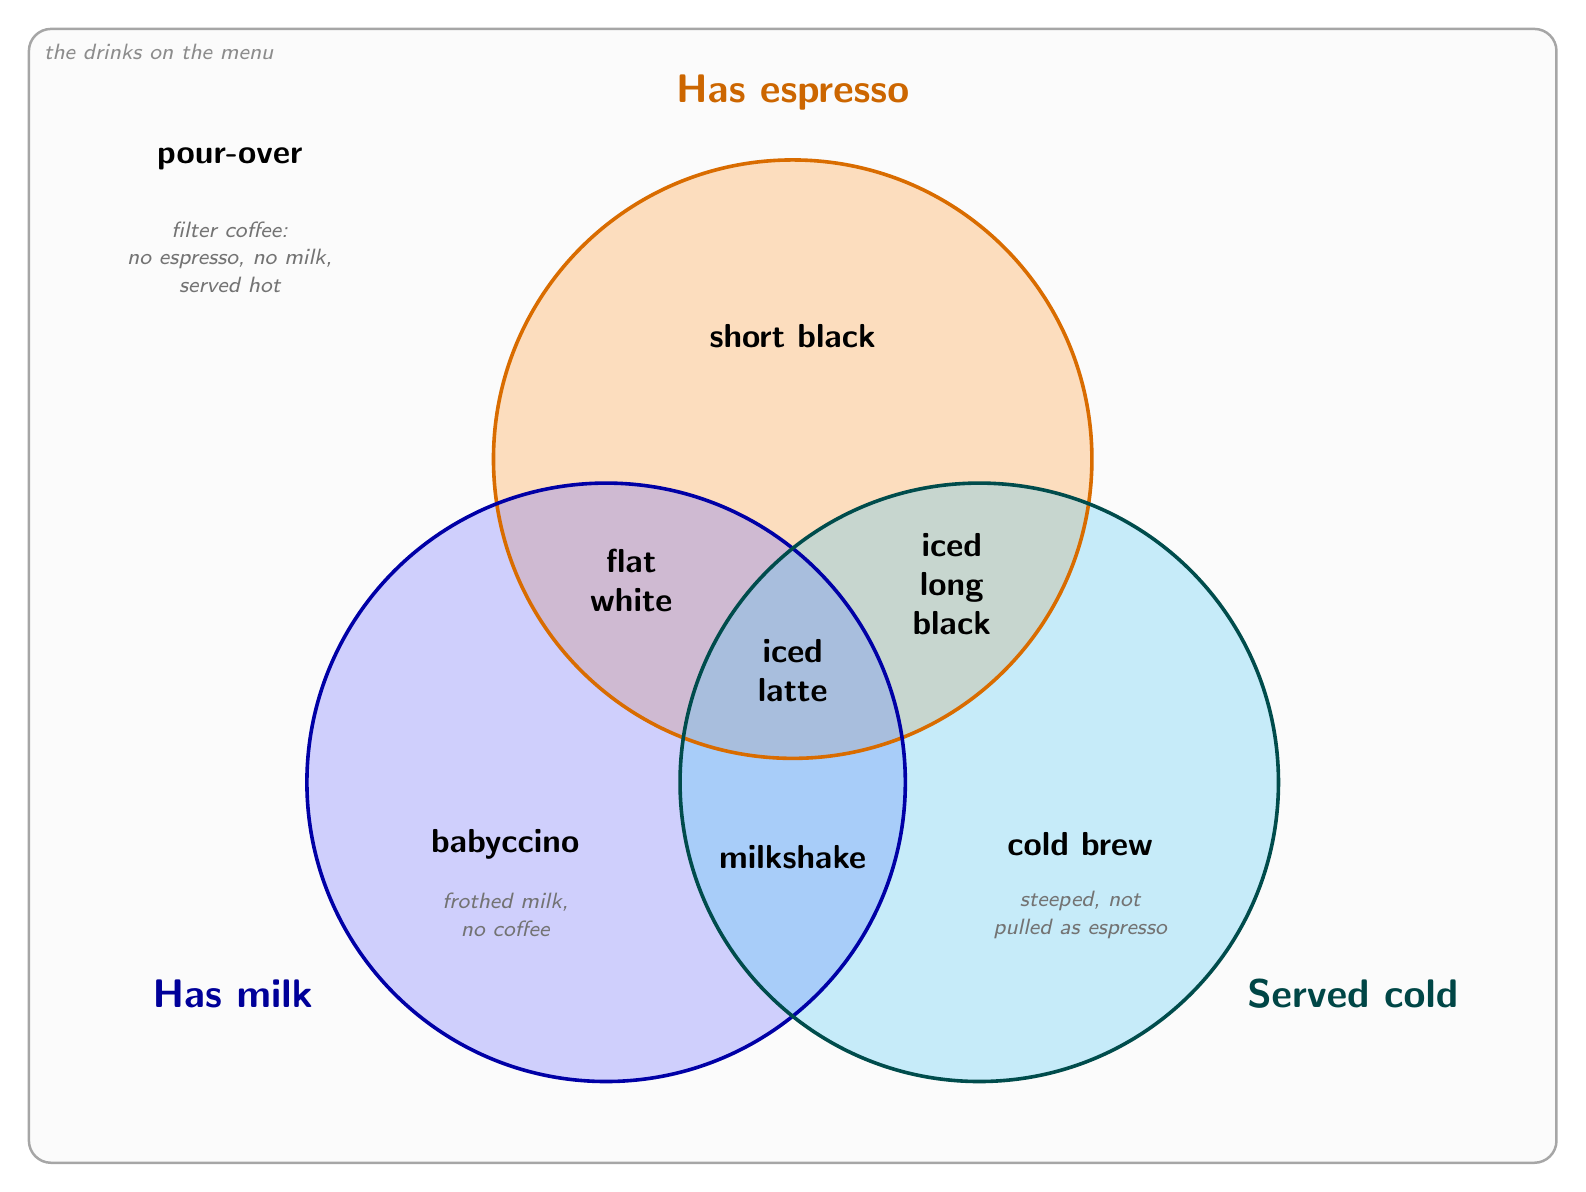
\begin{tikzpicture}[
    drink/.style={font=\sffamily\bfseries\fontsize{12}{14}\selectfont, text=black, align=center, inner sep=1pt},
    hint/.style ={font=\sffamily\itshape\fontsize{8.5}{10}\selectfont, text=black!55, align=center, inner sep=1pt},
    setlab/.style={font=\sffamily\bfseries\fontsize{14}{16}\selectfont, align=center, inner sep=2pt},
  ]

  % ---------------- geometry (tuned so every region can hold its text) -----
  \def\R{3.8}                                        % radius of each circle
  \def\C{2.736}                                      % distance of each centre from the origin
  \path (0,\C)   coordinate (cE)                     % "Has espresso"  -- top
        (210:\C) coordinate (cM)                     % "Has milk"      -- bottom left
        (330:\C) coordinate (cC);                    % "Served cold"   -- bottom right

  % ---------------- the rectangle of "all these drinks" --------------------
  \node[draw=black!35, line width=0.9pt, rounded corners=8pt, fill=black!1.5,
        minimum width=19.4cm, minimum height=14.4cm] at (0,1.0) {};
  \node[hint, anchor=north west, text=black!45] at (-9.55,8.05) {the drinks on the menu};

  % ---------------- three overlapping circles ------------------------------
  \begin{scope}[transparency group]
    \fill[orange!75, fill opacity=0.32] (cE) circle (\R);
    \fill[blue!55,   fill opacity=0.32] (cM) circle (\R);
    \fill[cyan!65,   fill opacity=0.32] (cC) circle (\R);
  \end{scope}
  \draw[orange!85!black, line width=1.3pt] (cE) circle (\R);
  \draw[blue!65!black,   line width=1.3pt] (cM) circle (\R);
  \draw[teal!60!black,   line width=1.3pt] (cC) circle (\R);

  % ---------------- names of the three sets, outside each circle -----------
  \node[setlab, text=orange!80!black, anchor=south]      at ($(cE)+(90:\R+0.55)$)  {Has espresso};
  \node[setlab, text=blue!60!black,   anchor=25]         at ($(cM)+(210:\R+1.05)$) {Has milk};
  \node[setlab, text=teal!55!black,   anchor=155]        at ($(cC)+(330:\R+1.05)$) {Served cold};

  % ---------------- the drinks ---------------------------------------------
  % espresso only  (hot, no milk)
  \node[drink] at (0,4.30)      {short black};
  % milk only      (no coffee at all)
  \node[drink] at (-3.65,-2.15) {babyccino};
  \node[hint]  at (-3.65,-3.05) {frothed milk,\\no coffee};
  % cold only      (cold, but never an espresso shot)
  \node[drink] at (3.65,-2.15)  {cold brew};
  \node[hint]  at (3.65,-3.05)  {steeped, not\\pulled as espresso};
  % espresso + milk, served hot
  \node[drink] at (-2.05,1.20)  {flat\\white};
  % espresso + cold, no milk
  \node[drink] at (2.02,1.15)   {iced\\long\\black};
  % milk + cold, no espresso
  \node[drink] at (0,-2.32)     {milkshake};
  % all three
  \node[drink] at (0,0.05)      {iced\\latte};

  % none of the three: hot filter coffee
  \node[drink, anchor=center] at (-7.15,6.55) {pour-over};
  \node[hint,  anchor=center] at (-7.15,5.30) {filter coffee:\\no espresso, no milk,\\served hot};

\end{tikzpicture}
\end{document}
